\documentclass[10pt]{beamer}
\usetheme[subsectionpage=progressbar]{metropolis}
\setbeamertemplate{section in toc}[sections numbered]
\setbeamertemplate{subsection in toc}[subsections numbered]
\metroset{progressbar=frametitle}
\metroset{numbering=none}
%W\usepackage[utf8]{inputenc}
\usepackage{ragged2e}
\usepackage{caption}
\usepackage{amsmath}
\usepackage[mathrm=sym]{unicode-math}
\setmathfont{Fira Math}
\usepackage{graphicx} 
\usepackage{appendixnumberbeamer}
\usepackage{booktabs}
\usepackage[font=small,labelfont=bf]{caption}
\usepackage{hyperref}
\usepackage[scale=2]{ccicons}
\usepackage{caption}
\usepackage{subcaption}

\usepackage{pgfplots}
\usepgfplotslibrary{dateplot}
\setsansfont[BoldFont={Fira Sans Bold}]{Fira Sans Book}
\usepackage{xspace}
\newcommand{\themename}{\textbf{\textsc{metropolis}}\xspace}
\theoremstyle{definition}
\metroset{block=fill}

\definecolor{Purple}{HTML}{911146}
\definecolor{Orange}{HTML}{CF4A30}
\setbeamercolor{alerted text}{fg=Orange}
\setbeamercolor{frametitle}{bg=Orange}
\renewcommand<>{\alert}[1]{\begin{alertenv}\bfseries#2#1\end{alertenv}}

\title{Detecting influential beliefs in large-scale surveys}
\date{July 2021}
\author{Aleksandar Tomašević}
\institute{University of Novi Sad}
%\titlegraphic{\hfill\includegraphics[height=1.9cm]{ff.pdf}}
\hbadness=99999
\begin{document}

\begin{frame}
    \titlepage
\end{frame}


  \begin{frame}
  \tableofcontents[hideallsubsections]
  \end{frame}


\section{Problem definition}

\section{Belief networks}

{\setbeamercolor{background canvas}{bg=white} \begin{frame}
  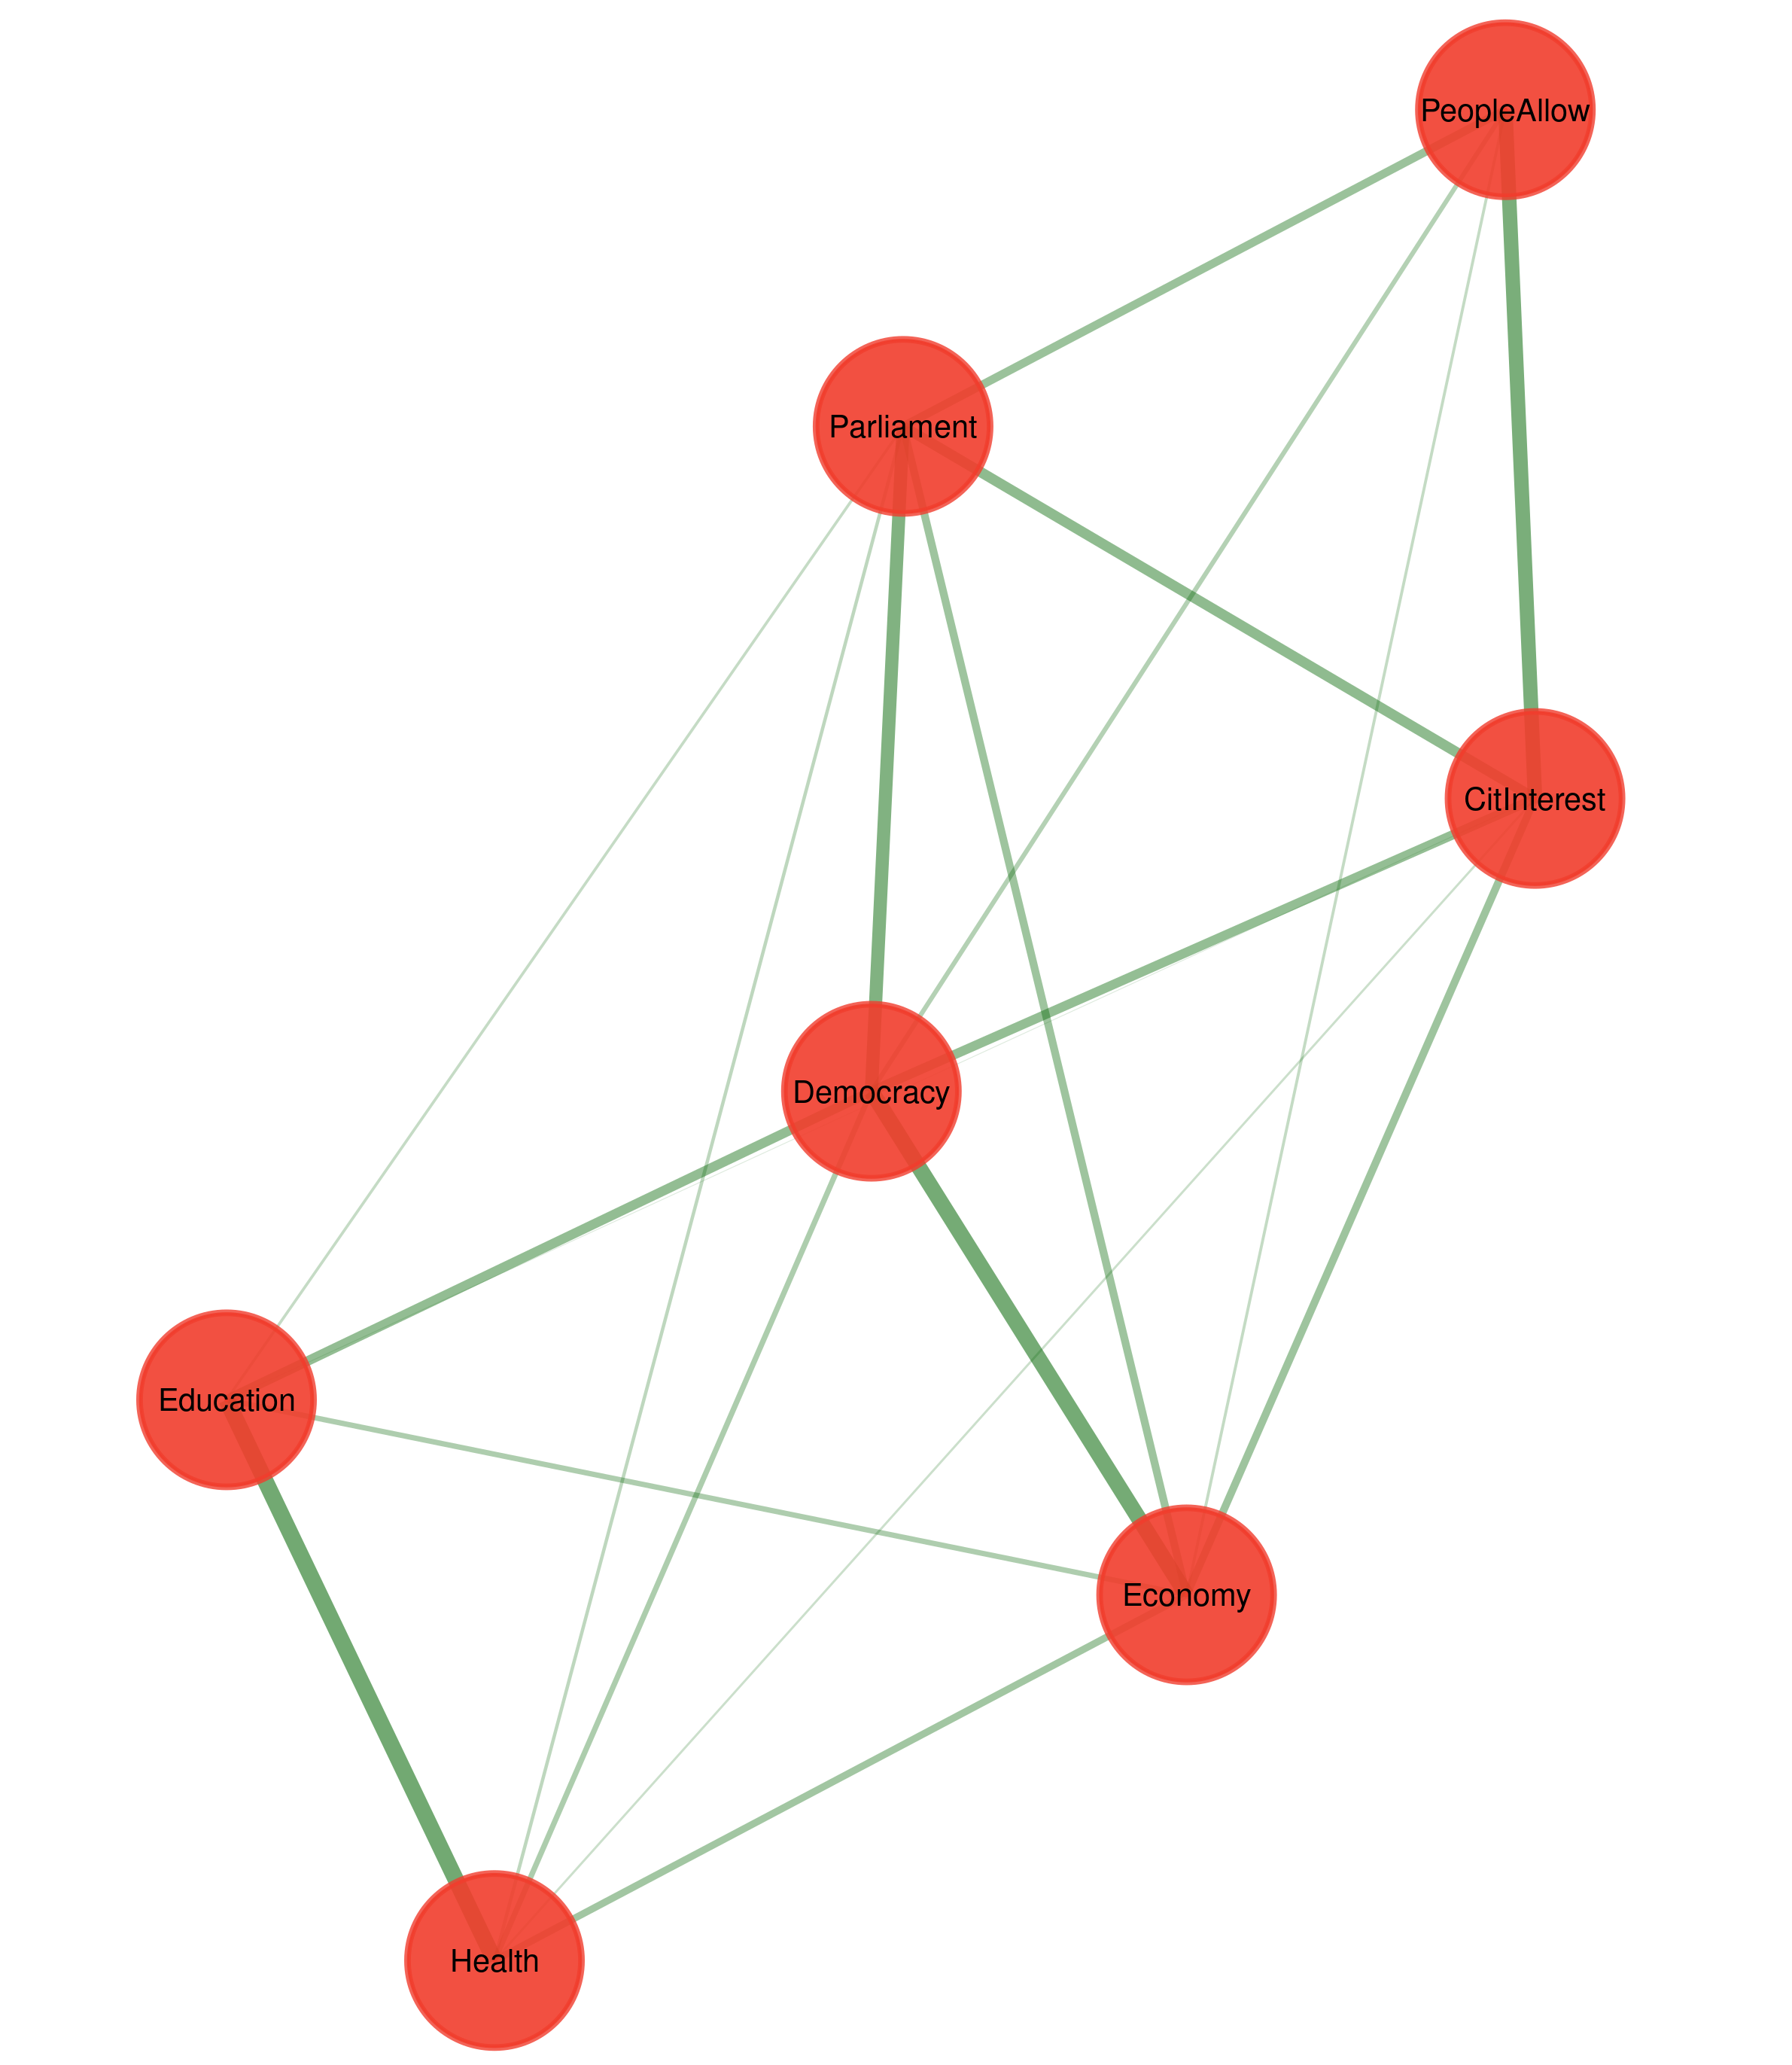
\includegraphics[width=0.65\paperwidth]{../figures/01-ega-full.png}
\end{frame}}

{\setbeamercolor{background canvas}{bg=white} \begin{frame}{\hspace{1cm}Electoral autocracies \hspace{1cm} VS \hspace{1cm} Liberal Democracies}
  \begin{figure}
  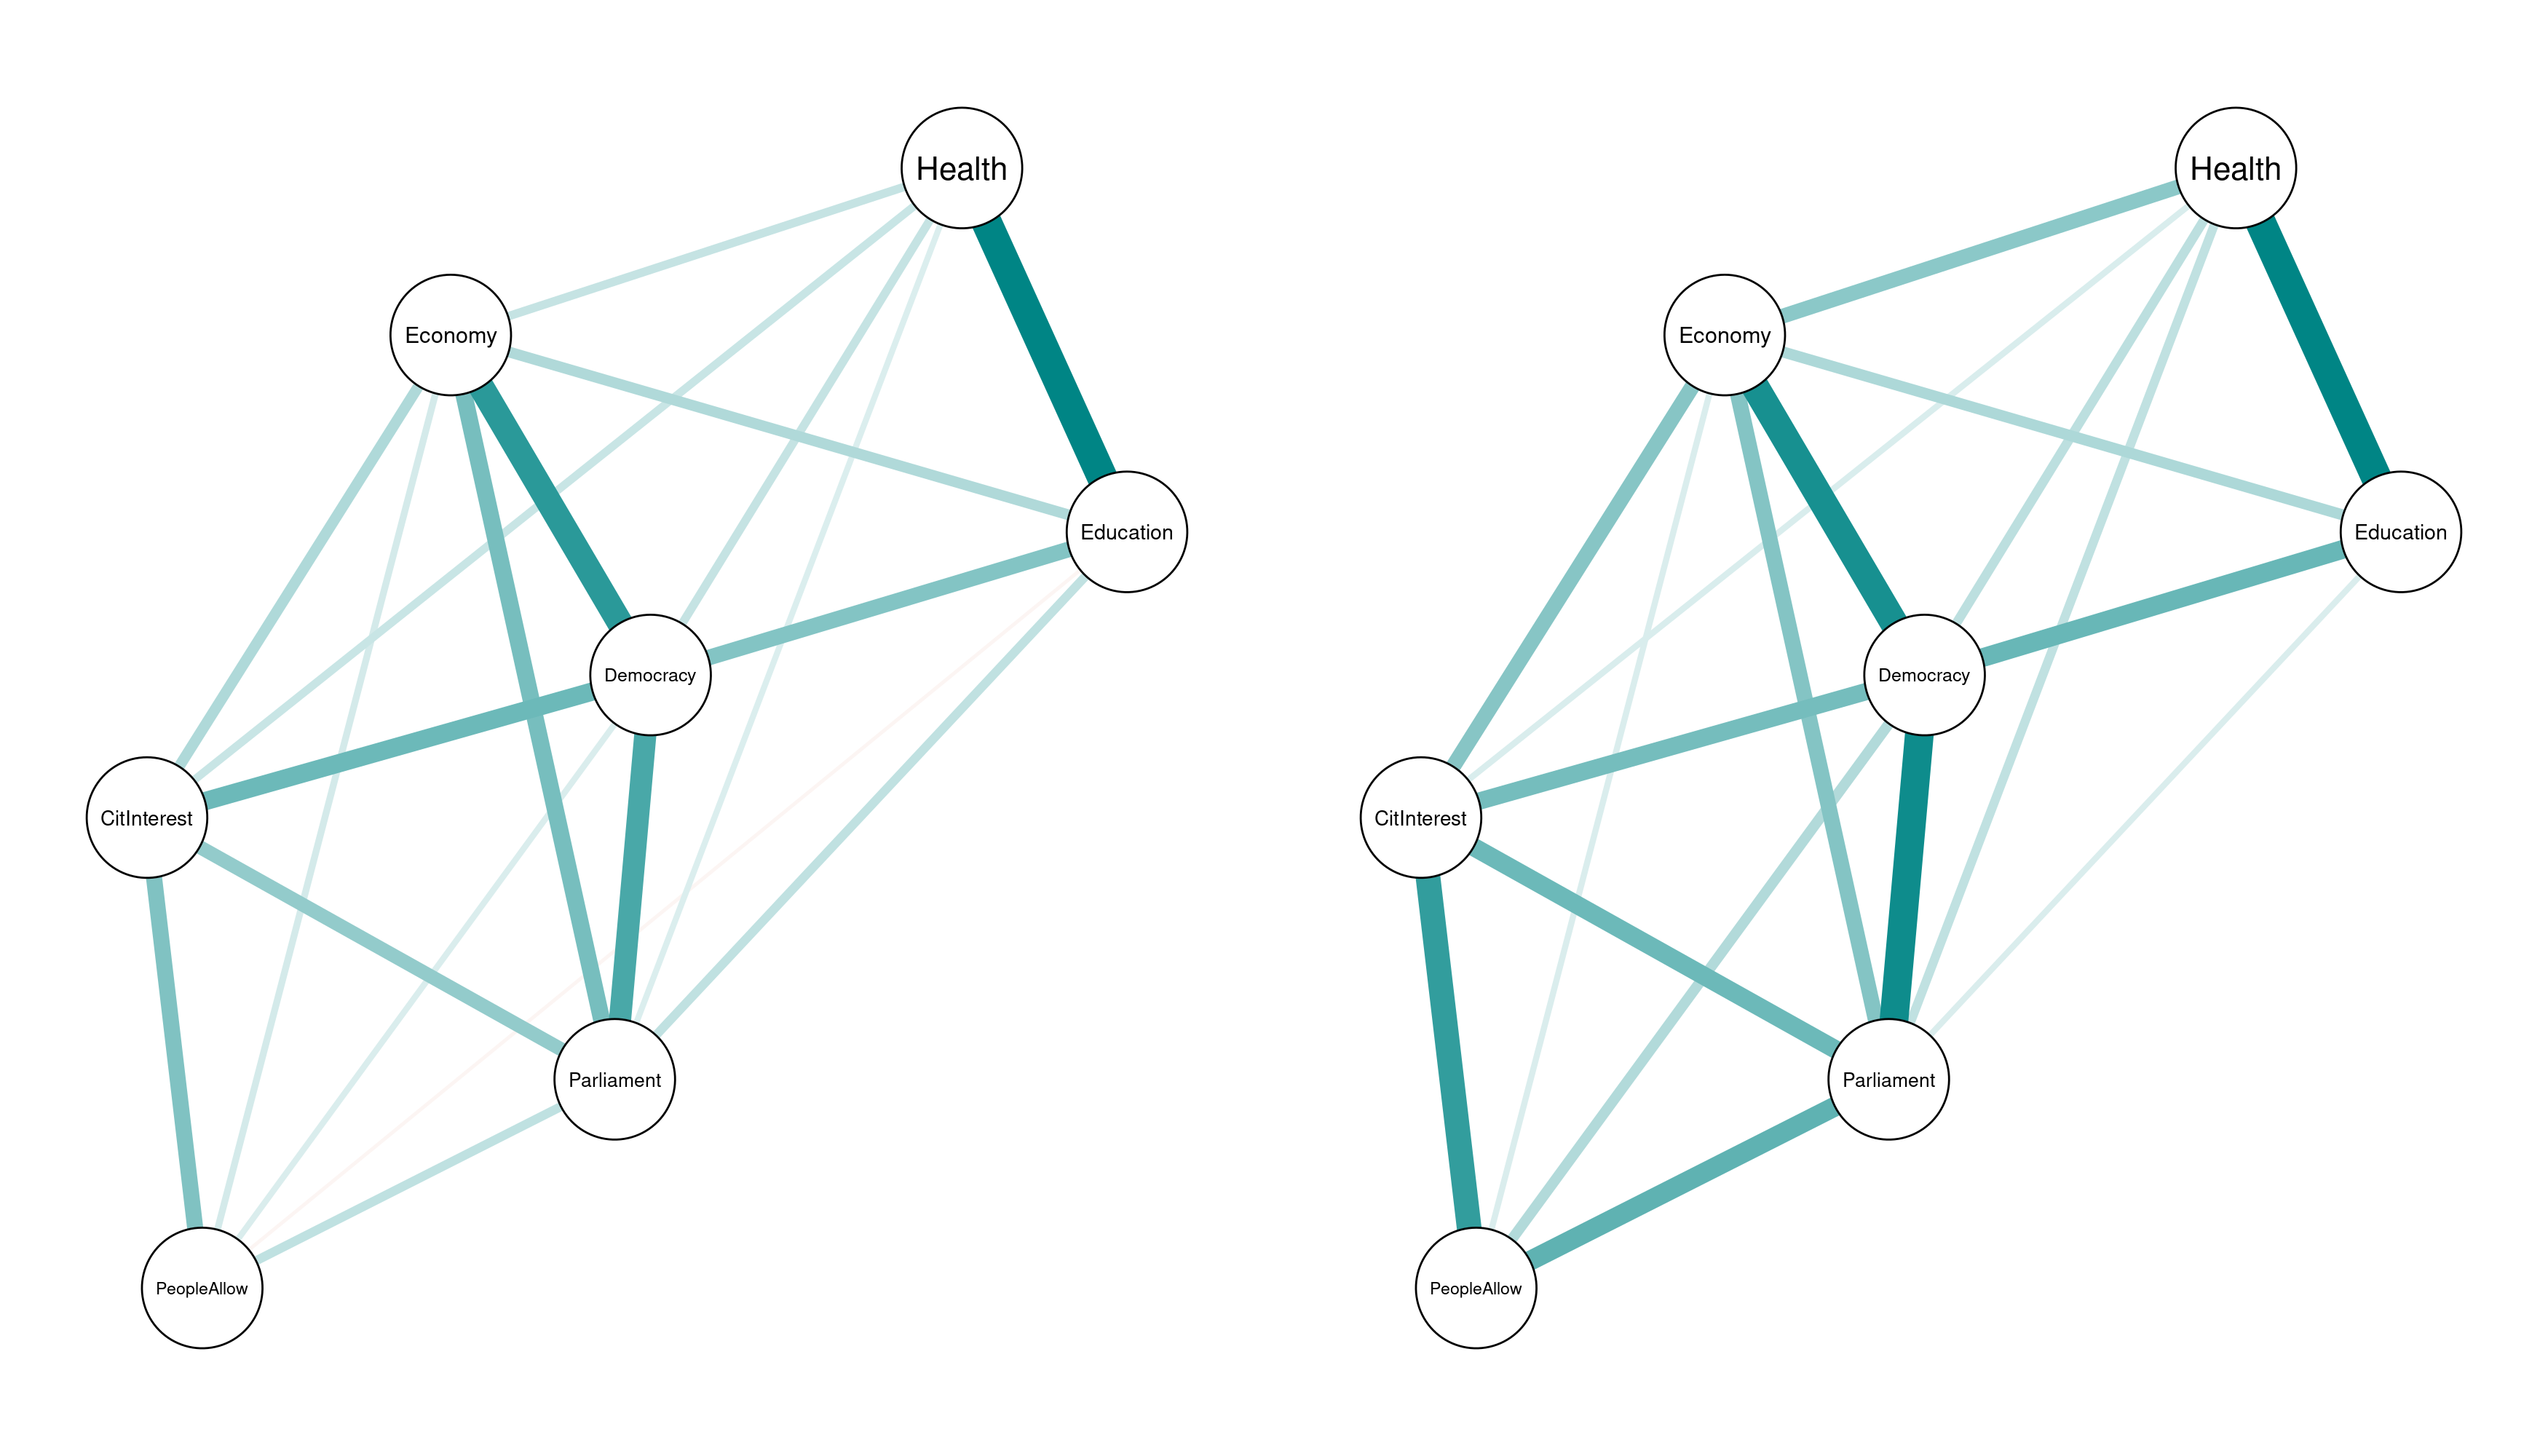
\includegraphics[width=0.95\paperwidth]{../figures/99-tree-ea-vs-ld.png}
  \end{figure}
\end{frame}}


\end{document}